%! Author = Wojciech Kot - 151879
% Preamble
\documentclass[11pt]{article}

% Packages
\usepackage{amsmath}
\usepackage[a4paper, margin=0.5in]{geometry}
\usepackage{graphicx} % daj an 1in jak chcesz normalniejszy margines, ale kod mi się w linii nie mieści :P
\usepackage[utf8]{inputenc}
\usepackage[T1]{fontenc}
\usepackage[polish]{babel}
\usepackage{float}
\usepackage{hyperref}
\usepackage{cleveref}
% \usepackage{subfigure}

\title{Raport ze studium przypadku}
\author{Wojciech Kot 151879}
\date{}

\begin{document}

\maketitle
\newpage

\section{Wstęp}\label{sec:wstep}

Zbiór danych, który zdecydowałem się przebadać to zbiór dostępny pod linkiem:
\href{https://www.kaggle.com/datasets/anandshaw2001/video-game-sales}{video-game-sales}.
Pochodzi on z serwisu kaggle i zawiera on informacje dotyczące sprzedaży gier wideo na różnych platformach sprzętowych,
w różnych regionach świata i w rozmaitych gatunkach gier.
Dane te mogą być wykorzystane zarówno do analizy trendów rynkowych,
jak i do przewidywania sprzedaży w zależności od cech gry, w tym takich jak jej wydawca, platforma, czy rok wydania.
Sam jestem ciekawy powiązań jakie (możliwe, że) uda się odkryć,
chociażby korelacji wydawcy ze sprzedażą i pewnych różnic pomiędzy wydawcami a sprzedażą w konkretnych rejonach świata.

\section{Opis zbioru danych}\label{sec:opis-zbioru-danych}

Zbiór danych składa się z \textbf{11 kolumn} i \textbf{16\,598 rekordów}.
Każdy rekord odpowiada jednej grze wideo na konkretnej platformie — oznacza to,
że jeśli dana gra została wydana na kilku platformach (np.\ PC i PS4),
to pojawia się w zbiorze danych wielokrotnie, jako osobne wpisy dla każdej z tych platform.

Każdy rekord zawiera następujące atrybuty:
\begin{itemize}
  \item \textbf{Rank} – pozycja gry w globalnym rankingu sprzedaży,
  \item \textbf{Name} – tytuł gry,
  \item \textbf{Platform} – platforma, na której gra została wydana (np. PC, PS4),
  \item \textbf{Year} – rok wydania gry,
  \item \textbf{Genre} – gatunek gry (np. Action, Sports),
  \item \textbf{Publisher} – wydawca gry,
  \item \textbf{NA\_Sales} – sprzedaż w Ameryce Północnej (w milionach egzemplarzy),
  \item \textbf{EU\_Sales} – sprzedaż w Europie (w milionach egzemplarzy),
  \item \textbf{JP\_Sales} – sprzedaż w Japonii (w milionach egzemplarzy),
  \item \textbf{Other\_Sales} – sprzedaż w pozostałych regionach świata (w milionach egzemplarzy),
  \item \textbf{Global\_Sales} – łączna sprzedaż na całym świecie (w milionach egzemplarzy).
\end{itemize}

Zbiór zawiera również brakujące wartości. \\
\textbf{Publisher} ma 58 brakujących wartości, oraz \\
\textbf{Year} ma 271 brakujących wartości.

\section{Eksploracja danych}\label{sec:eksploracja-danych}

\subsection{Histogramy zmiennych ilościowych}\label{subsec:histogramy-zmiennych-ilosciowych}

Dla wszystkich zmiennych ilościowych (w tym sprzedaży regionalnej i globalnej) wygenerowałem histogramy.
Analiza wykazała silne skośności w rozkładach -- zdecydowana większość gier osiąga bardzo niską sprzedaż (poniżej 0.5 miliona egzemplarzy),
natomiast tylko nieliczne tytuły mają sprzedaż przekraczającą 5 milionów.
Sugeruje to obecność efektu długiego ogona typowego dla rynku gier, jak i dla ogółu rynków produktów rozrywkowych.

\begin{figure}[H]
    \centering
    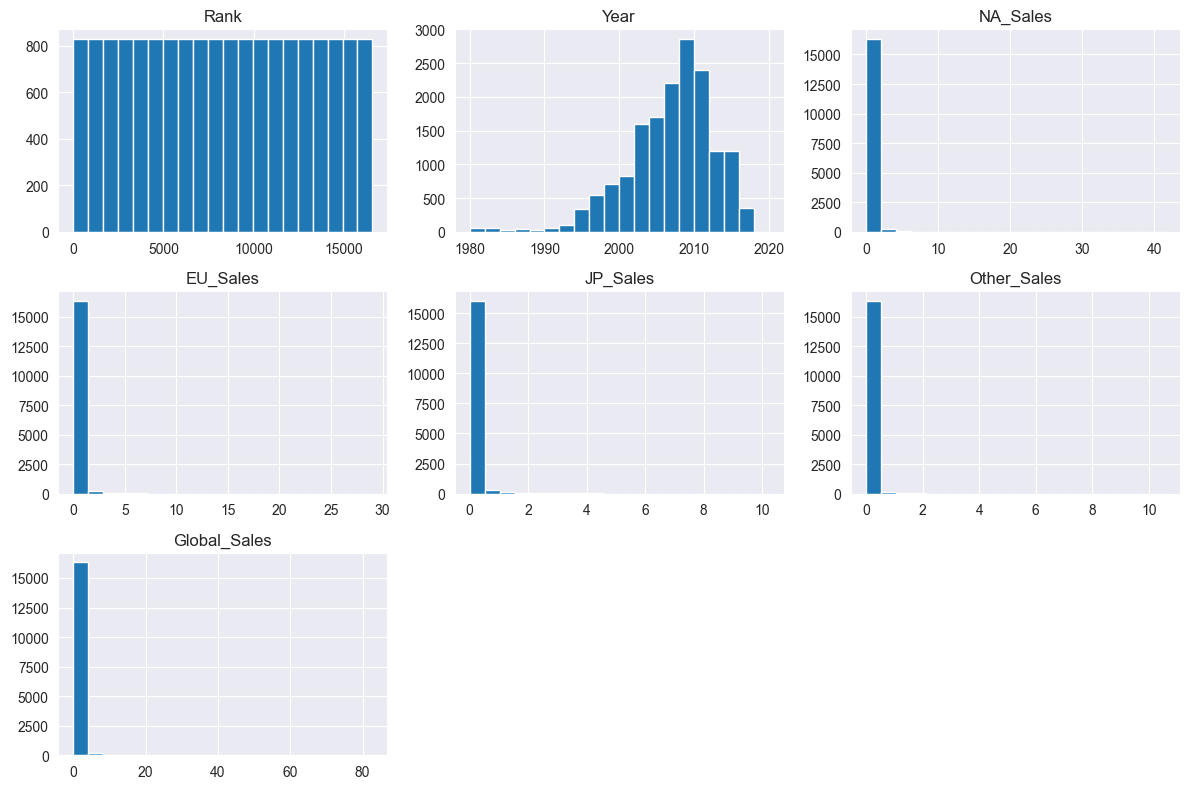
\includegraphics[width=0.5\linewidth]{figures/histogramy}
    \caption{Histogramy przedstawiające rozkład danych}
    \label{fig:histogramy}
\end{figure}

\subsection{Analiza korelacji}\label{subsec:analiza-korelacji}

Obliczyłem macierz korelacji pomiędzy zmiennymi ilościowymi i przedstawiam ją graficznie jako heatmapę.
Najsilniejsze korelacje zaobserwowano między regionalnymi sprzedażami a \texttt{Global\_Sales},
co jest zgodne z intuicją – wartości te są składnikami łącznej sprzedaży.
W szczególności:
\begin{itemize}
  \item \texttt{NA\_Sales} i \texttt{Global\_Sales}: wysoka dodatnia korelacja,
  \item \texttt{EU\_Sales} i \texttt{Global\_Sales}: wysoka dodatnia korelacja,
  \item \texttt{JP\_Sales} – znacznie niższa stosunkowo korelacja z resztą regionów, co może wskazywać na odrębność rynku japońskiego.
\end{itemize}

Po obliczeniu korelacji, należy zwrócić uwagę na rynek japoński.
Wygląda na to, że nie podąża on do końca za światowym trendem,
a niska korelacja sugeruje, że mogą panować na nim zupełnie inne trendy.

\begin{figure}[H]
    \centering
    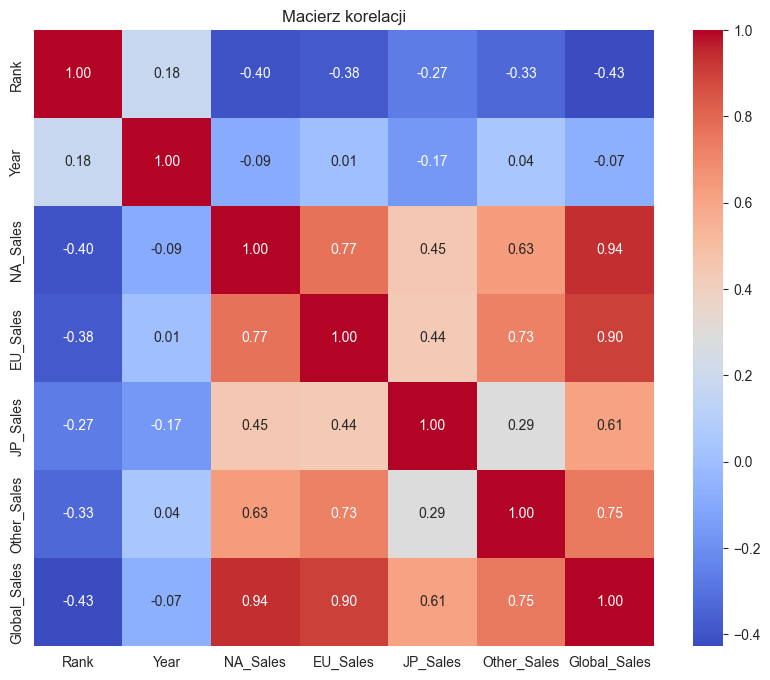
\includegraphics{figures/korelacje}
    \caption{Korelacja pomiędzy atrybutami liczbowymi}
    \label{fig:korelacje}
\end{figure}

\subsection{Sprzedaż w czasie}\label{subsec:sprzedaz-w-czasie}

Zbadałem również rozkład sprzedaży gier w kolejnych latach.
Dane pokazują wzrost liczby wydawanych gier oraz ich sprzedaży począwszy od lat 90.,
z wyraźnym szczytem w okolicach roku 2008, po którym obserwowany jest stopniowy spadek.
Spadek ten może wynikać zarówno z faktycznego zmniejszenia liczby wydań, jak i niepełności danych w późniejszych latach.
Z własnej wiedzy jestem w stanie stwierdzić, że głównym powodem tego spadku będą brakujące dane,
szczególnie braki w latach 2020 i późniejszych, kiedy rynek gier miał swego rodzaju ``złotą erę''.
Niestety, nie udało mi się znaleźć podobnie holistycznych danych co do sprzedaży gier po 2015 roku.
Mimo to, bazując na licznych medialnych doniesieniach z branży gier wideo z kolejnych lat wnioskuję że wynikiem widocznego spadku są brakujące dane względem rzeczywistości.

\begin{figure}[H]
    \centering
    \begin{minipage}[t]{0.48\linewidth}
        \centering
        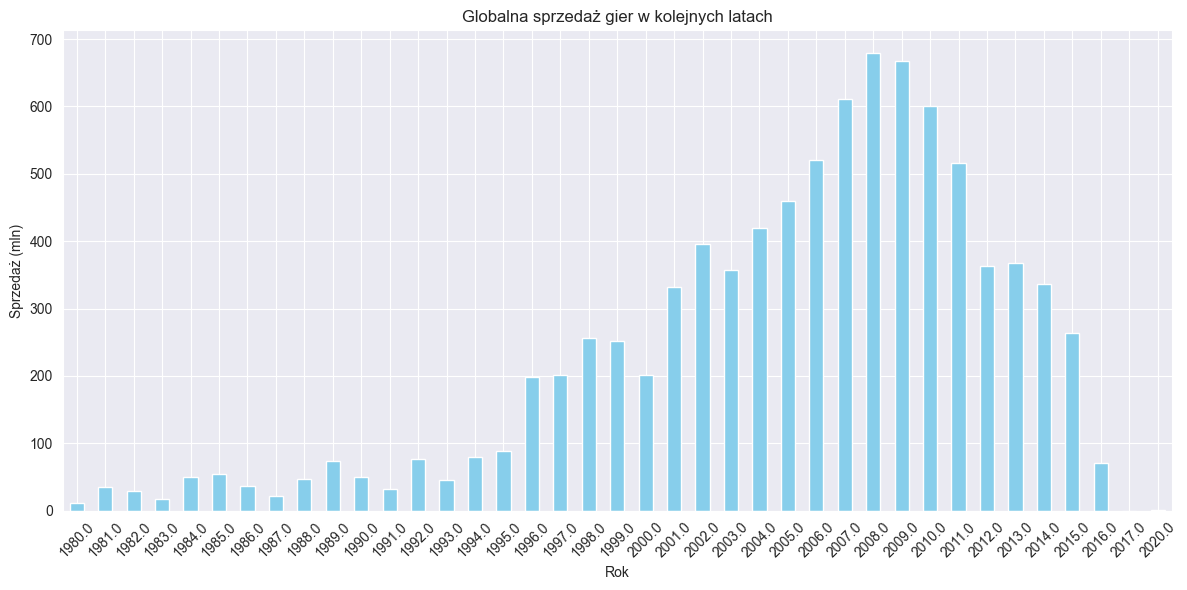
\includegraphics[width=\linewidth]{figures/Lata-sprzedaz}
        \caption{Sprzedaż w mln \$ w kolejnych latach}
        \label{fig:sprzedaz}
    \end{minipage}
    \hfill
    \begin{minipage}[t]{0.48\linewidth}
        \centering
        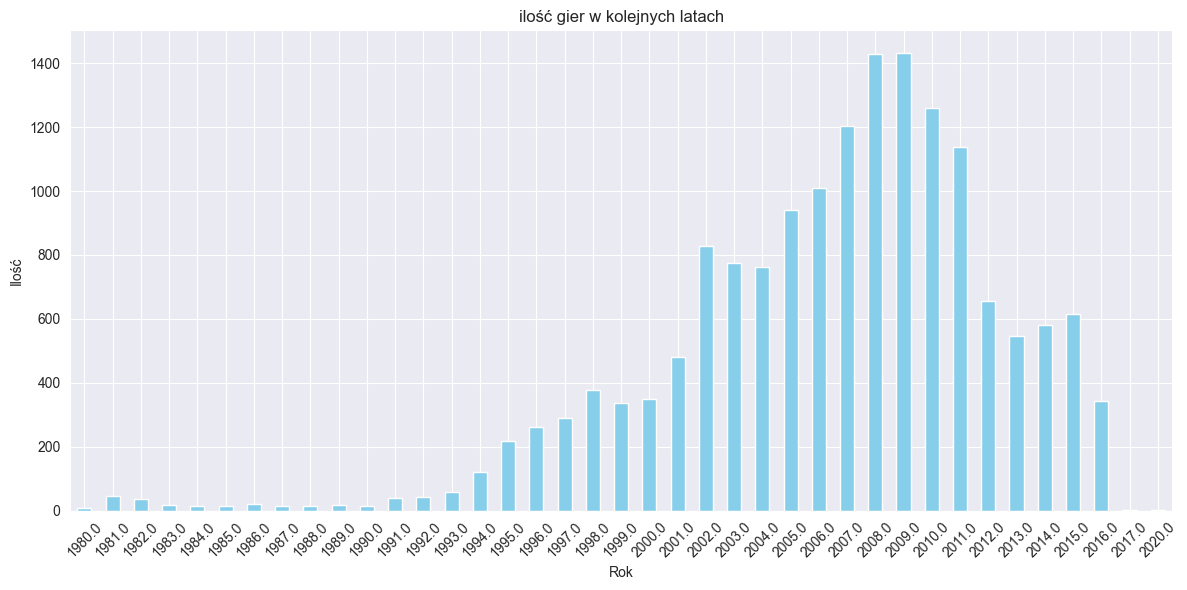
\includegraphics[width=\linewidth]{figures/Lata-ilosc}
        \caption{Ilośc gier sprzedanych w kolejnych latach}
        \label{fig:sprzedaz2}
    \end{minipage}
\end{figure}


\subsection{Badanie wydawców}\label{subsec:badanie-wydawcow}

Badając zbiór danych przeanalizowałem też pewne własności konkretnych wydawców.
Przede wszystkim, zdecydowałem się zbadać jakie są najpopularniejsze gatunki dla danych wydawców, czyli czy istnieje pewna korelacja, a jeśli tak, to jaka, pomiędzy wydawcą a gatunkiem.

\begin{figure}[H]
    \centering
    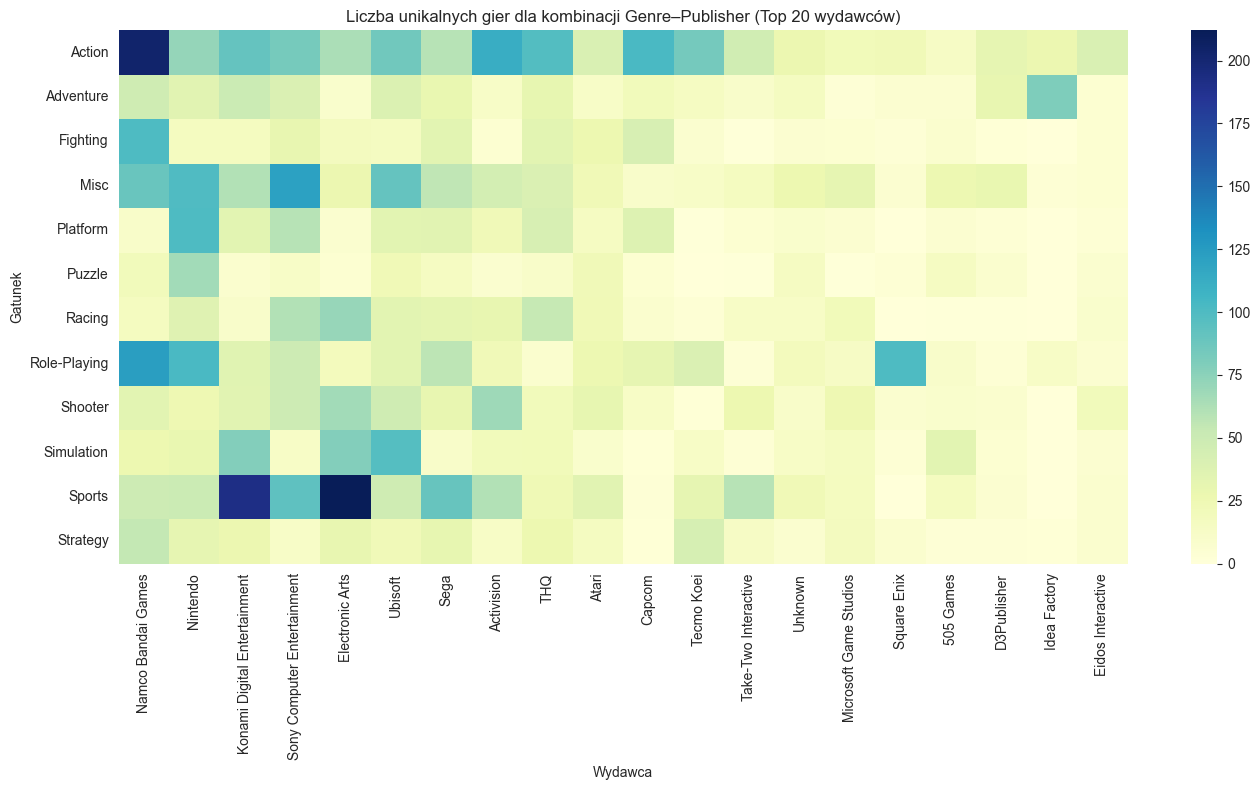
\includegraphics[width=0.9\linewidth]{figures/Genre-Publisher}
    \caption{Liczba unikalnych gier z danego gatunku, dla danych wydawców}
    \label{fig:wydawcy0}
\end{figure}

Dodatkowo, chciałem zobaczyć czy występują różnice pomiędzy ilością wydawanych gier, a zyskiem z ich sprzedaży, stąd 3 zestawienia na wykresach~\ref{fig:wydawcy_all}
\begin{figure}[H]
    \centering
    \begin{minipage}[t]{0.48\linewidth}
        \centering
        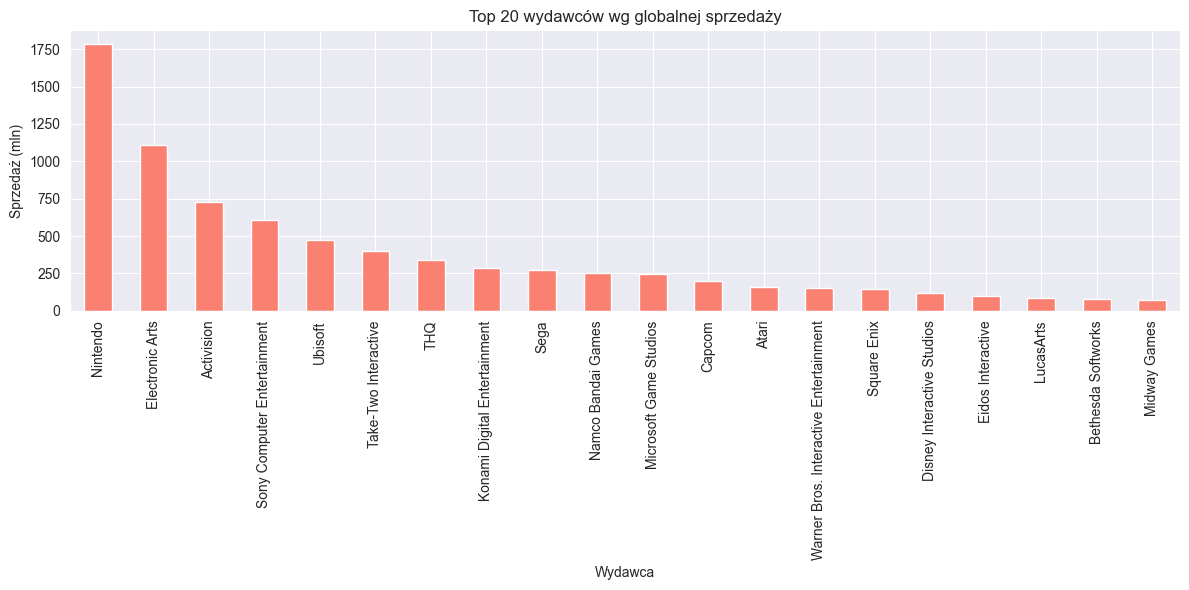
\includegraphics[width=\linewidth]{figures/wydawcy-sprzedaz}
    \end{minipage}
    \hfill
    \begin{minipage}[t]{0.48\linewidth}
        \centering
        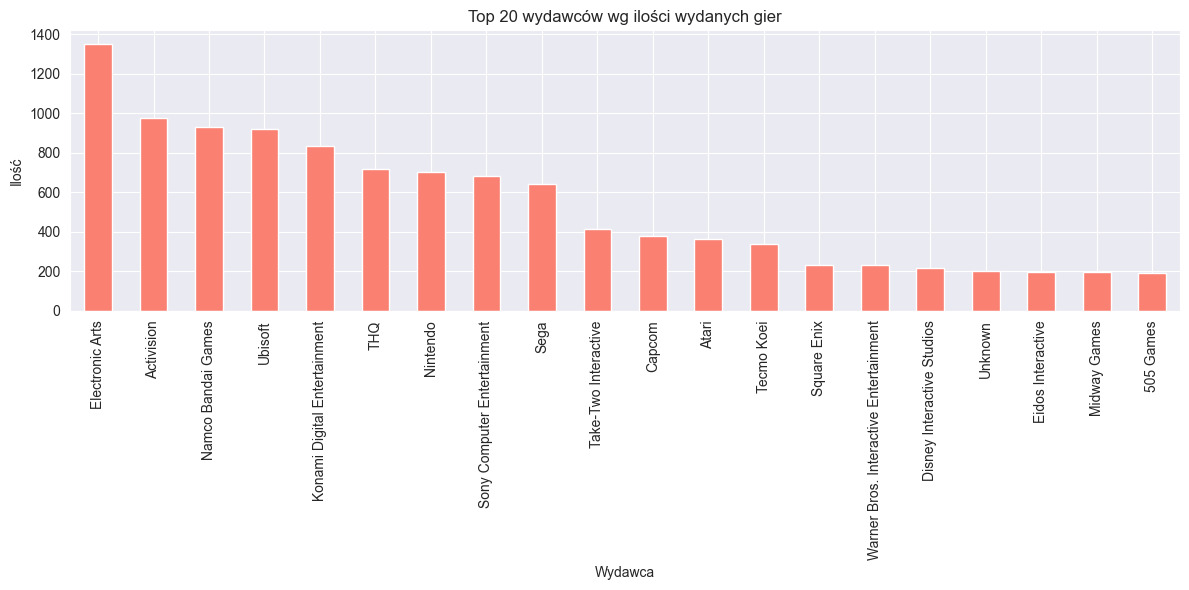
\includegraphics[width=\linewidth]{figures/wydawcy-ilosc}
    \end{minipage}

    \vspace{0.5em}

    \begin{minipage}[t]{0.6\linewidth}
        \centering
        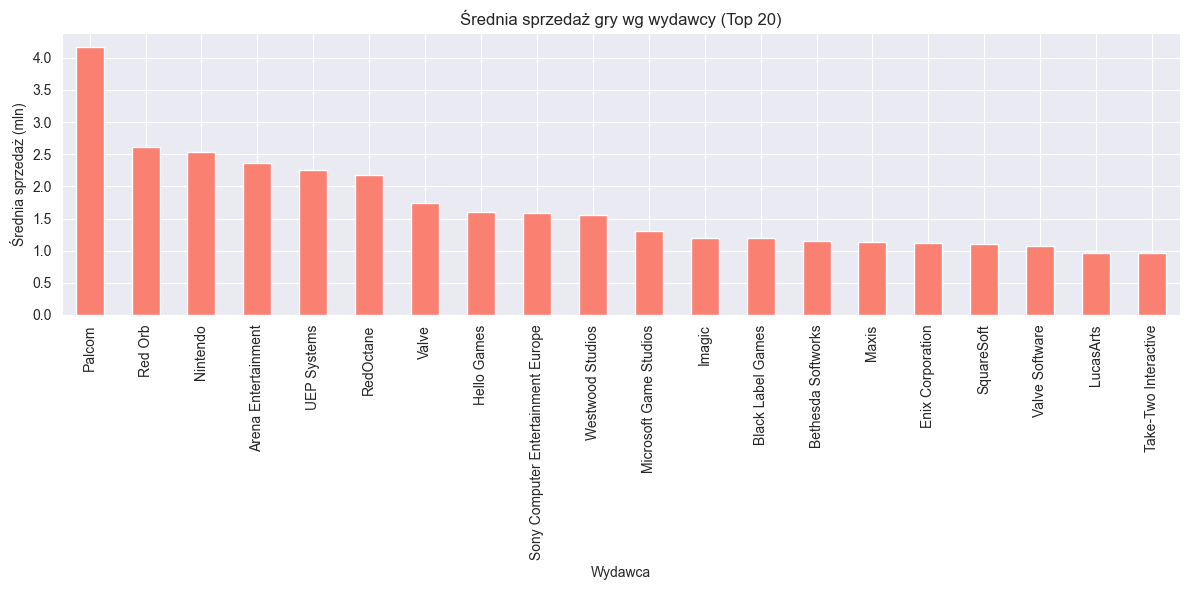
\includegraphics[width=\linewidth]{figures/wydawcy-srednia-sprzedaz}
    \end{minipage}

    \caption{Top 20 wydawców według globalnej sprzedaży (góra lewa), liczby wydanych gier (góra prawa) oraz średniej sprzedaży (dół)}
    \label{fig:wydawcy_all}
\end{figure}

Same te zestawienia prowokują myśli o tym, w jaki sposób powinno się kategoryzować wydawców, czy faworyzować ``dużych graczy''
przez największe zarobki (wynikające często z tego, jak dużo gier wydają), czy może skorzystać ze średniej sprzedaży,
potencjalnie faworyzując wydawców jednego lub dwóch hitów, ale nie znanych szerszej publiczności poza danymi tytułami.

\subsection{Badanie gatunków}\label{subsec:badanie-gatunkow}
Badając dalej zbiór danych zdecydowałem się przyjrzeć bliżej gatunkom gier występującym w datasecie.
Istnieje tutaj gatunek ``Misc'' oznaczający tyle co gatunek ``Inny'' (z ang.~ Miscellaneous).
Jest on o tyle ciekawym przypadkiem, że pomimo bycia trzecim najczęstszym gatunkiem, nie odzwierciedla tego wcale sprzedaż globalna dla tego gatunku, jak widać na~\ref{fig:gat} oraz na~\ref{fig:gat2}.

\begin{figure}[H]
    \centering
    \begin{minipage}[t]{0.48\linewidth}
        \centering
        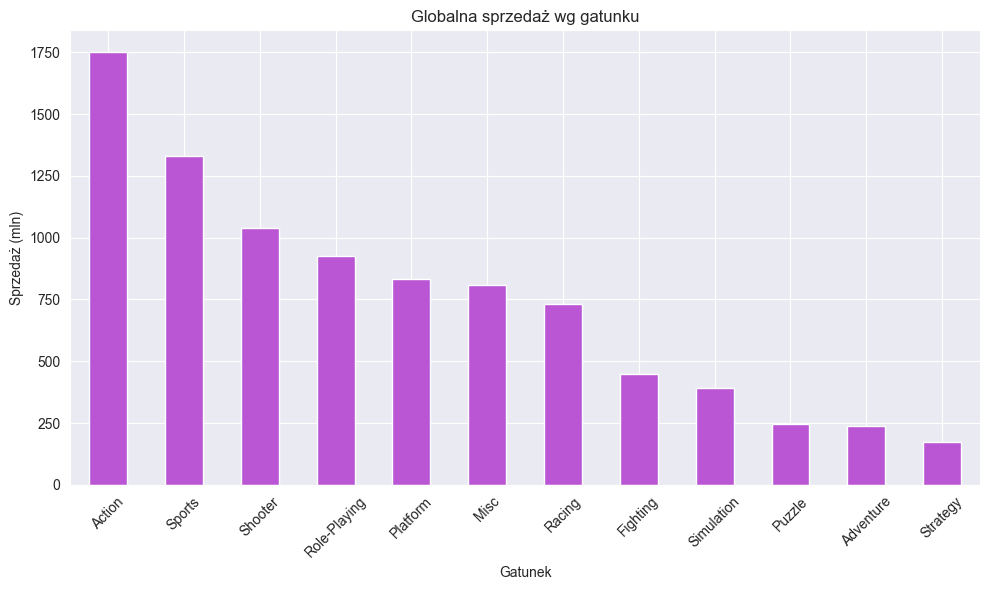
\includegraphics[width=\linewidth]{figures/gatunek-sprzedaz}
        \caption{Sprzedaż w mln \$ dla danych gatunków}
        \label{fig:gat}
    \end{minipage}
    \hfill
    \begin{minipage}[t]{0.48\linewidth}
        \centering
        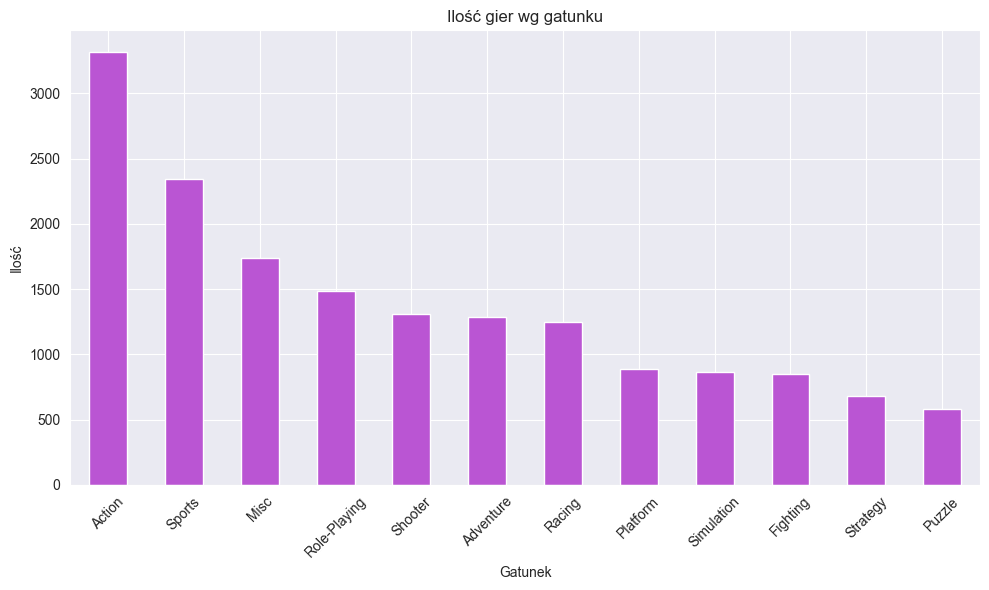
\includegraphics[width=\linewidth]{figures/gatunek-ilosc}
        \caption{Ilość gier wydanych dla danych gatunków}
        \label{fig:gat2}
    \end{minipage}
\end{figure}


\subsection{Badanie platform}\label{subsec:badanie-platform}
Najciekawsze z wniosków przyniosło mi badanie zależności między platformami.
Początkowo, wykonałem podobne zestawienia jak powyżej:

\begin{figure}[H]
    \centering
    \begin{minipage}[t]{0.48\linewidth}
        \centering
        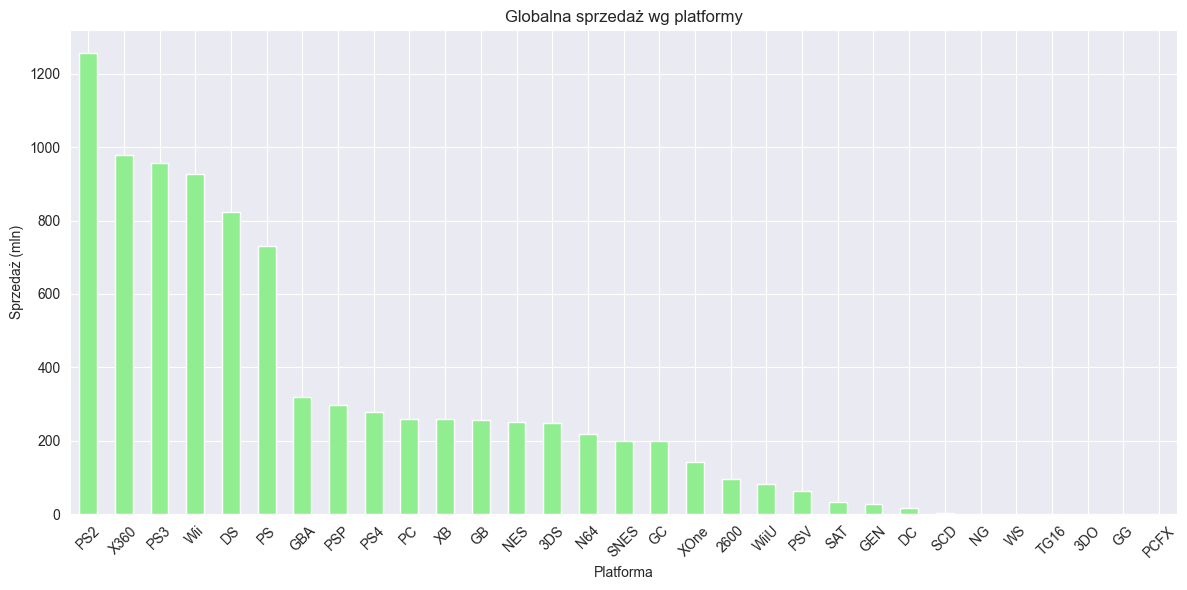
\includegraphics[width=\linewidth]{figures/platforma-sprzedaz}
        \caption{Sprzedaż w mln \$ na danej platformie}
        \label{fig:platform}
    \end{minipage}
    \hfill
    \begin{minipage}[t]{0.48\linewidth}
        \centering
        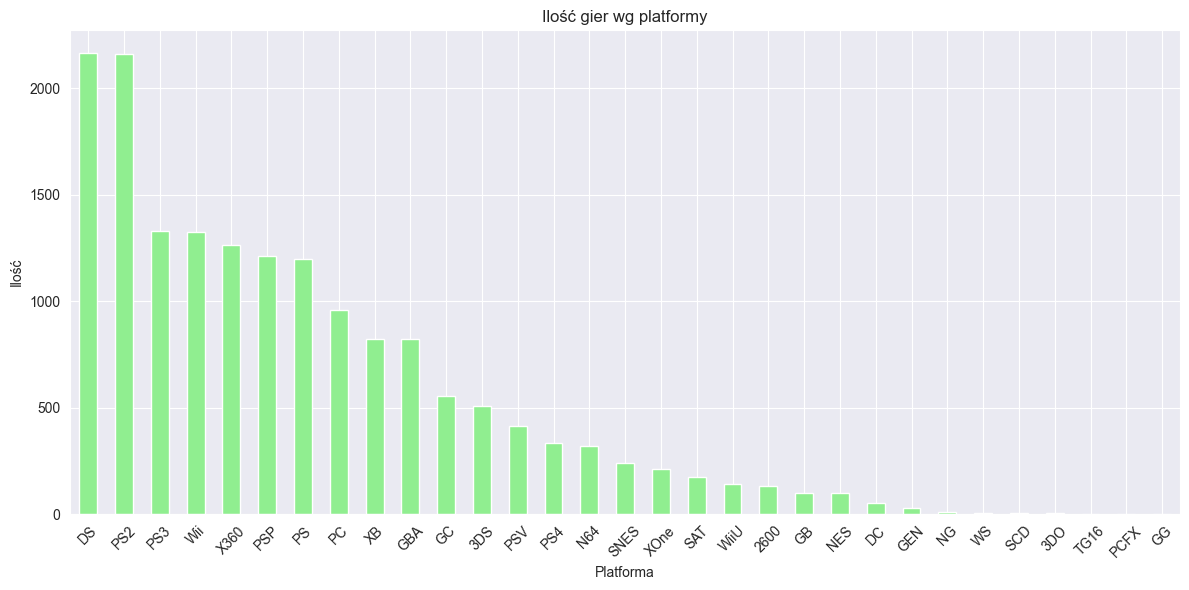
\includegraphics[width=\linewidth]{figures/platforma-ilosc}
        \caption{Ilość gier wydanych na danej platformie}
        \label{fig:platform2}
    \end{minipage}
\end{figure}

Jednak to nie koniec, bo znacznie więcej informacji można wyciągnąć z zestawienia sprzedaży (czy to ilości gier, czy \$) dla platform w danym roku, za pomocą heatmapy.

\begin{figure}[H]
    \centering
    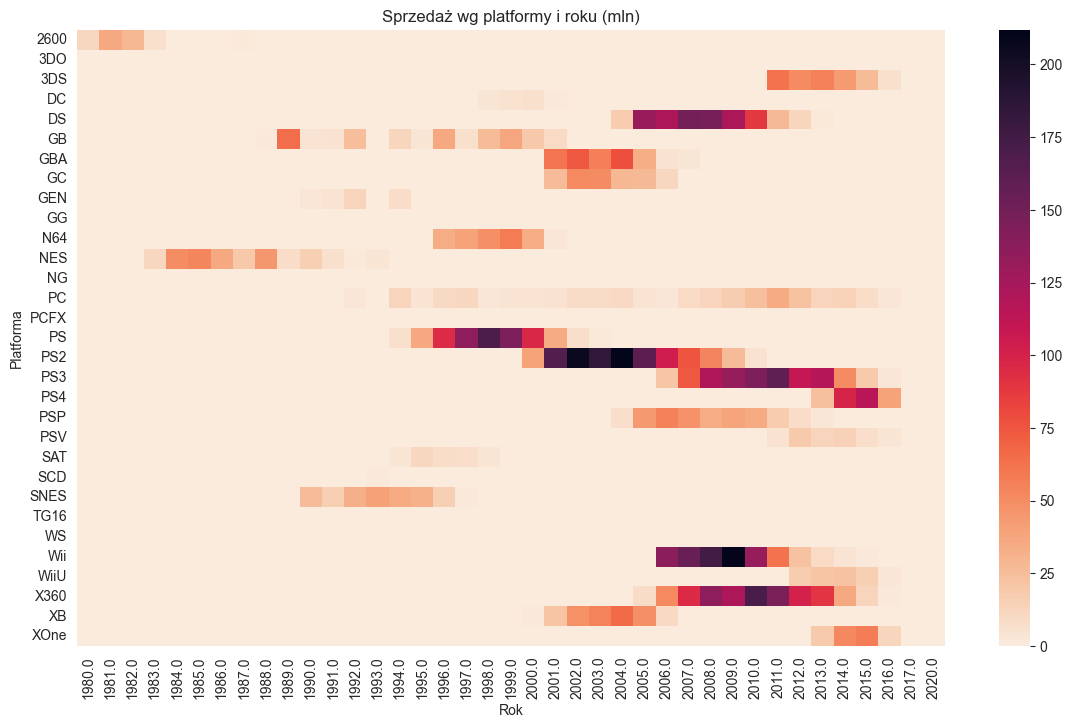
\includegraphics[width=\linewidth]{figures/rokplatforma-sprzedaz}
    \caption{Sprzedaż gier według platformy i roku}
    \label{fig:platform-year-sales}
\end{figure}

\begin{figure}[H]
    \centering
    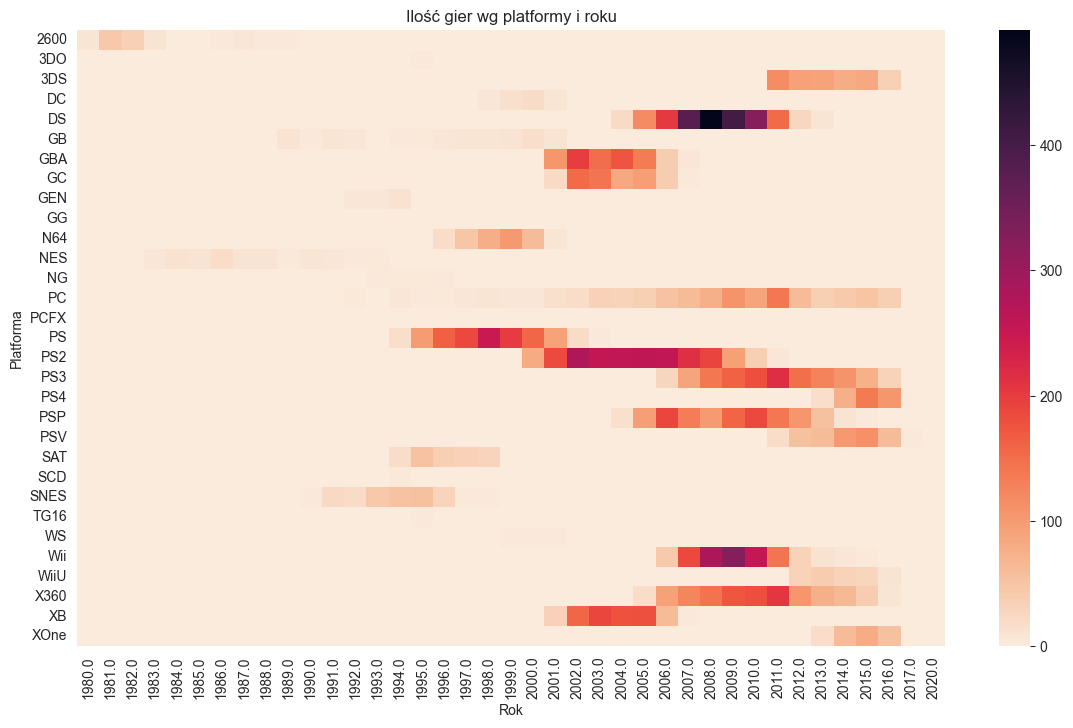
\includegraphics[width=\linewidth]{figures/rokplatforma-ilosc}
    \caption{Ilość gier wydanych według platformy i roku}
    \label{fig:platform-year-count}
\end{figure}

Przede wszystkim nasuwają się oczywiste wnioski, że żadna z badanych platform nie ma długiego życia.
Co roku właściwie pojawiały się na rynku nowe platformy, podbierając część klientów od ``głównych graczy'', aby za jakiś czas zostać wypartymi z rynku przez inne, nowsze platformy do gry.
Szczególnie widać to po serii PlayStation, gdzie gdy w 2000.~roku pojawia się PS2, to sprzedaż dla PS znacznie maleje na rzecz wzrostu tej na nowej generacji.
Ostatnie lata przedstawione na wykresie mogą być skrzywione ze względu na brakujące dane, wspomniane znacznie wcześniej w tym raporcie.
Biorąc to pod uwagę, można zauważyć wyjątkowo długie ``życie'' platformy PC - co ma przełożenie również i w 2025 roku, gdzie gry wideo na komputerach, zamiast na dedykowanych konsolach, nadal są bardzo popularne.
Głównym czynnikiem może być to, że w przypadku PC nie wyznacza się generacji, przez co nie ma ograniczeń technologicznych związanych z przestarzałą technologią.



\section{Modelowanie sprzedaży gier}\label{sec:modelowanie-sprzedazy-gier}

W celu przewidywania globalnej sprzedaży gier (\texttt{Global\_Sales}),
wytrenowałem kilka modeli regresyjnych, bazując na dostępnych cechach (rok, platforma, wydawca oraz gatunek.
Dane poddałem odpowiedniemu przetworzeniu: brakujące wartości zostały uzupełniłem bądź usunąłem (gdzie nie udało się znaleźć tych danych),
następnie przy użyciu one-hot encoding zakodowałem, a dane liczbowe znormalizowałem tam, gdzie było to wymagane.

Ocenę modeli opieram na czterech metrykach:\\
MAE - średni błąd bezwzględny\\
RMSE - pierwiastka z błędu średniokwadratowego\\
współczynnika \( R^2 \)\\
oraz MAPE - średniego procentowego błędu bezwzględnego.

\begin{table}[H]
\centering
\begin{tabular}{|l|c|c|c|c|}
\hline
\textbf{Model} & \textbf{MAE} & \textbf{RMSE} & \textbf{R\textsuperscript{2}} & \textbf{MAPE} \\
\hline
Regresja liniowa & 0.563 & 1.993 & 0.092 & 395.33\% \\
Drzewo regresji  & 0.583 & 2.103 & -0.012 & 514.01\% \\
XGBoost          & 0.531 & 1.988 & 0.096 & 395.26\% \\
\hline
\end{tabular}
\caption{Porównanie skuteczności modeli regresyjnych}
\label{tab:model_comparison}
\end{table}

Wszystkie trzy modele osiągają bardzo niskie wartości współczynnika determinacji \( R^2 \),
co oznacza, że praktycznie nie wyjaśniają zmienności globalnej sprzedaży.
Mimo że XGBoost nieznacznie przewyższa pozostałe podejścia, różnice są marginalne.
Ekstremalnie wysokie MAPE, jak i wysokie wartości RMSE wskazują,
że modele mają trudności z trafnym przewidywaniem wartości sprzedaży.

Zjawisko to może wynikać z braku istotnych danych w zbiorze — np.~jakości gry, marketingu, daty premiery względem świąt lub ówczesnej konkurencji rynkowej.

Mimo to zdecydowałem się zbadać ważność kryteriów, poprzez wizualizację drzewa, oraz wykres ważności cech w XGBoost:

\begin{figure}[H]
    \centering
    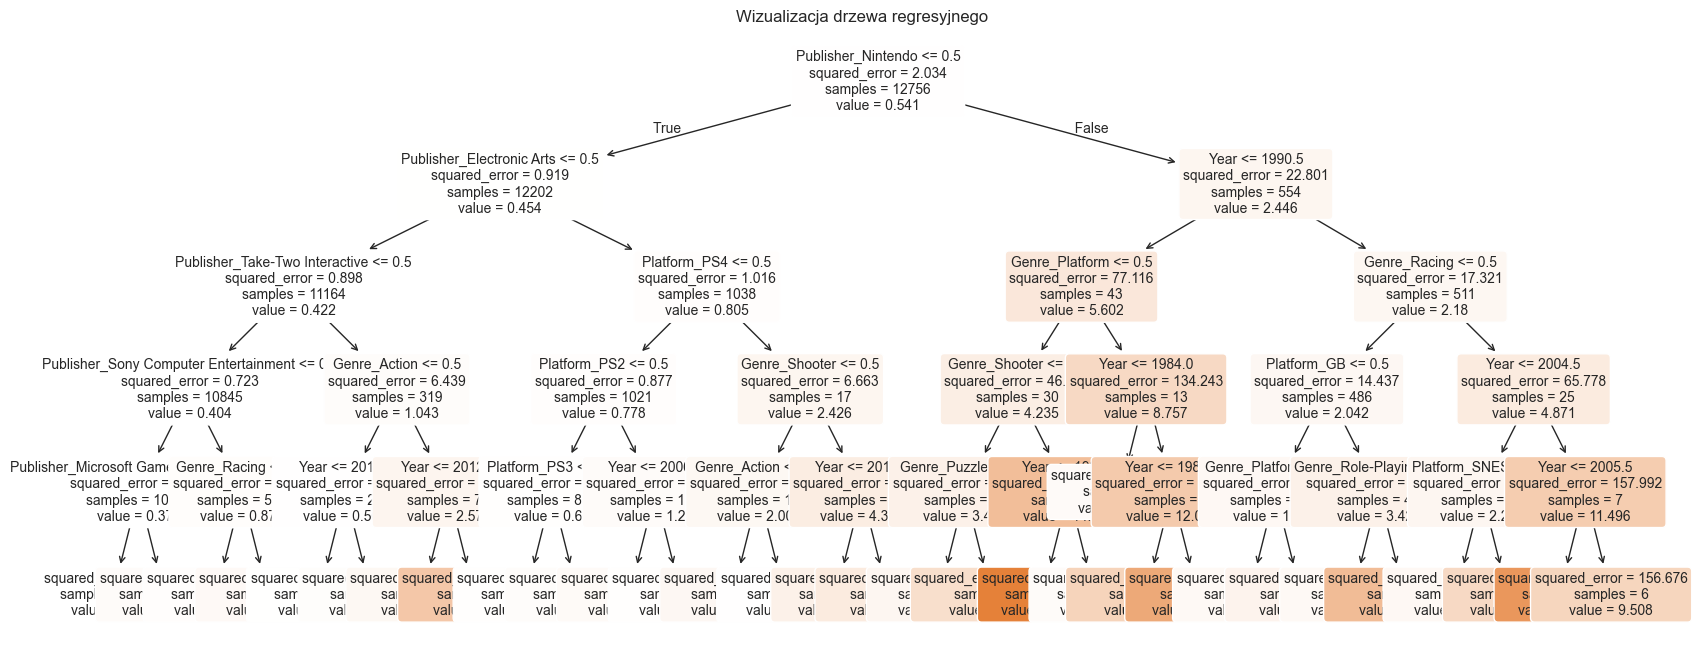
\includegraphics[width=0.9\linewidth]{figures/drzewo1}
    \caption{Wizualizacja drzewa decyzyjnygo}
    \label{fig:tree1}
\end{figure}

\begin{figure}[H]
    \centering
    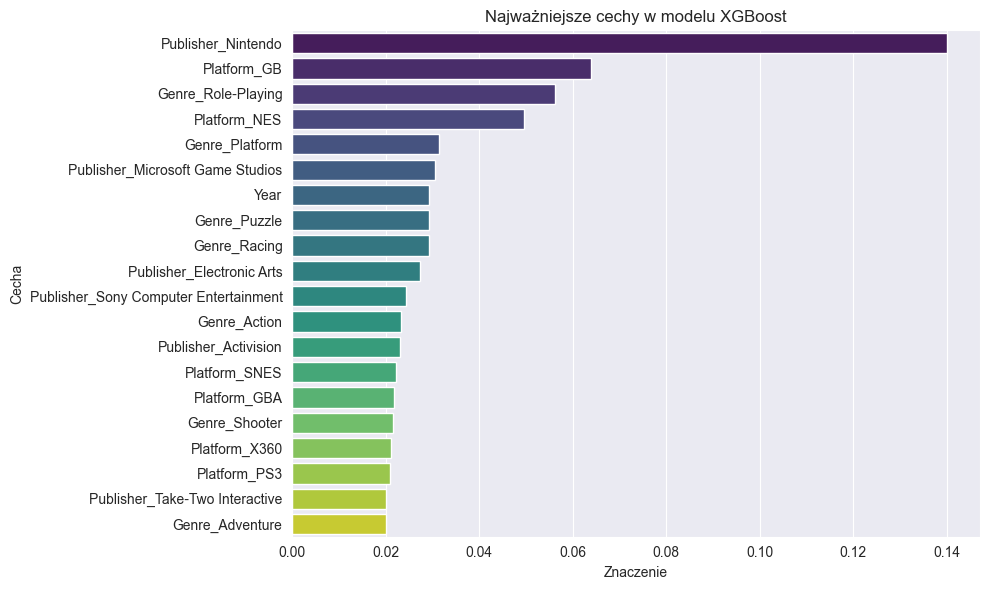
\includegraphics[width=0.9\linewidth]{figures/xgboost1}
    \caption{Ważność cech według modelu XGBoost}
    \label{fig:xgb_importance1}
\end{figure}


Moim kolejnym pomysłem było wytrenowanie podobnych modeli, ale tym razem dając im dostęp do cząstkowych danych o sprzedaży.
Oczywiście, bezsensowne jest dawanie modelom dostępu do wszystkich danych o cząstkowej sprzedaży, jednak z czystej ciekawości postanowiłem to zrobić mimochodem:

\begin{table}[H]
\centering
\begin{tabular}{|l|c|c|c|c|}
\hline
\textbf{Model} & \textbf{MAE} & \textbf{RMSE} & \textbf{R\textsuperscript{2}} & \textbf{MAPE} \\
\hline
Regresja liniowa & 0.003 & 0.005 & 1.000 & 3.16\% \\
Drzewo regresji  & 0.171 & 0.845 & 0.837 & 126.26\% \\
XGBoost          & 0.055 & 0.916 & 0.808 & 13.69\% \\
\hline
\end{tabular}
\caption{Porównanie skuteczności modeli regresyjnych}
\label{tab:model_comparison2}
\end{table}

Nawet tutaj, okazuje się, że model oparty o drzewo decyzyjne osiąga znacznie gorsze wyniki,
co było i nadal jest dla mnie zaskoczeniem.
Przy tak silnie skorelowanych danych, nawet XGBoost osiągnął gorsze wyniki od regresji liniowej,
ale nie ma się czemu dziwić, korelacja między składowymi a sumą jest oczywiście bardzo duża.

\begin{figure}[H]
    \centering
    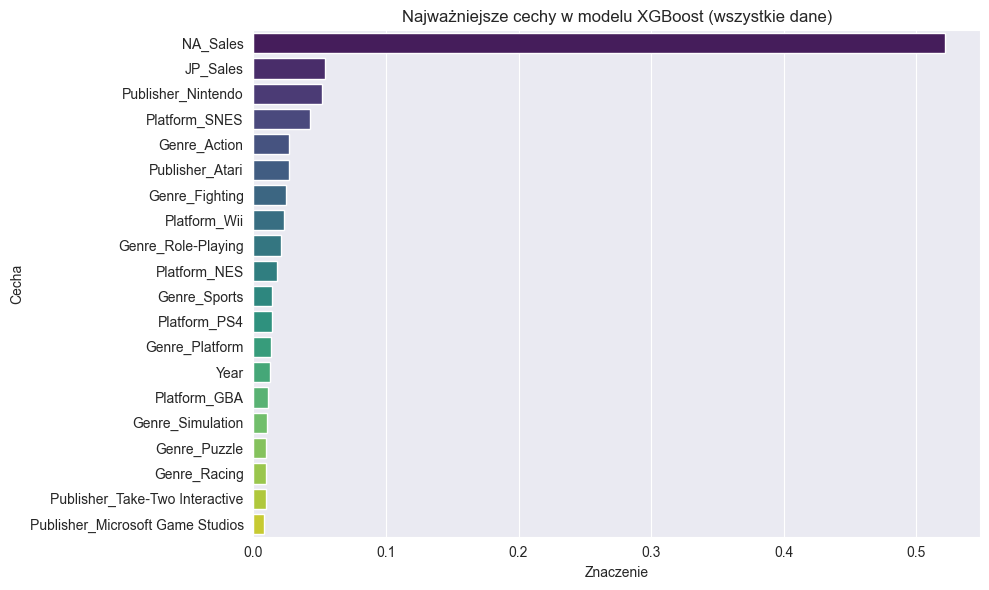
\includegraphics[width=0.9\linewidth]{figures/xgboost-all}
    \caption{Ważność cech według modelu XGBoost dla wszystkich danych}
    \label{fig:xgb_importance2}
\end{figure}

W przypadku pozostawienia jedynie dwóch znanych składowych, a więc sprzedaży w stanach~(\texttt{NA\_Sales}),
oraz sprzedaży w Japonii~(\texttt{Japan\_Sales}),
można stworzyć modele prognozujące sprzedaż globalną trochę dokładniej, chociaż najlepiej byłoby stworzyć takie,
które nie opierają się na żadnej cząstkowej sprzedaży.

\begin{table}[H]
\centering
\begin{tabular}{|l|c|c|c|c|}
\hline
\textbf{Model} & \textbf{MAE} & \textbf{RMSE} & \textbf{R\textsuperscript{2}} & \textbf{MAPE} \\
\hline
Regresja liniowa & 0.157 & 0.495 & 0.944 & 99.23\% \\
Drzewo regresji  & 0.200 & 0.909 & 0.811 & 125.08\% \\
XGBoost          & 0.145 & 1.113 & 0.717 & 59.42\% \\
\hline
\end{tabular}
\caption{Porównanie skuteczności modeli regresyjnych (na danych z USA i Japonii)}
\label{tab:model_comparison3}
\end{table}

\begin{figure}[H]
    \centering
    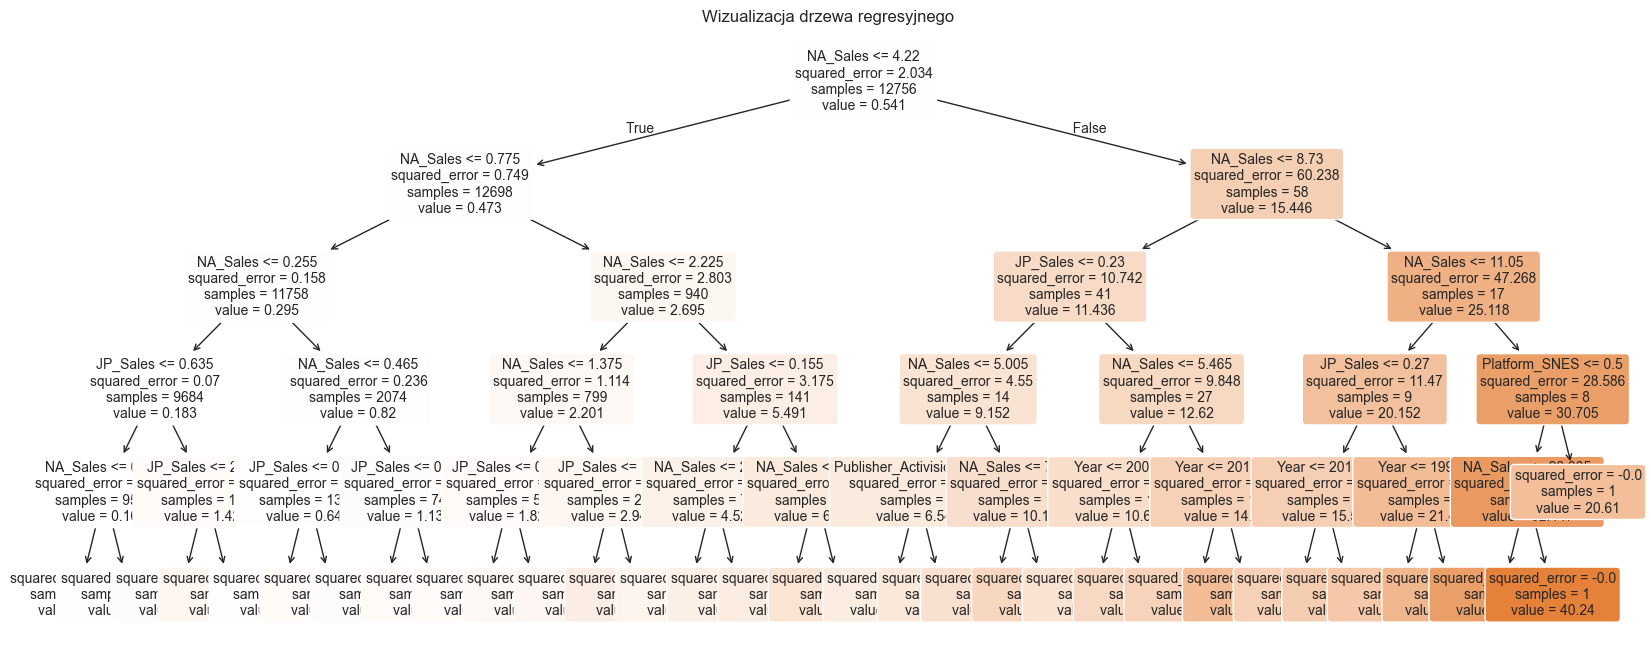
\includegraphics[width=0.9\linewidth]{figures/tree-last}
    \caption{Wizualizacja drzewa decyzyjnygo}
    \label{fig:tree-last}
\end{figure}

\begin{figure}[H]
    \centering
    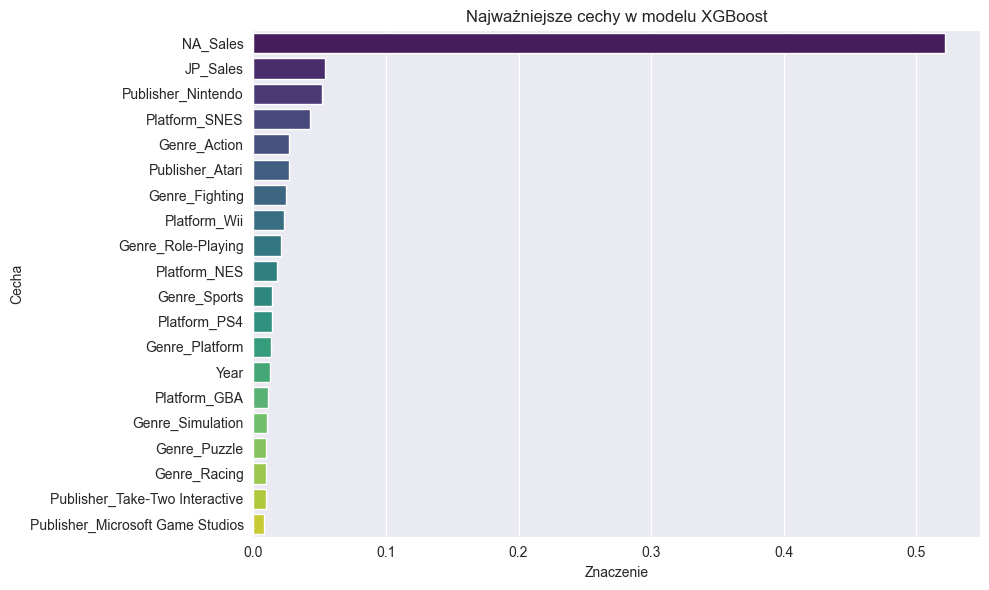
\includegraphics[width=0.9\linewidth]{figures/xgboost-last}
    \caption{Ważność cech według modelu XGBoost}
    \label{fig:xgb_importance-last}
\end{figure}

\section{Wnioski}\label{sec:wnioski}

TODO - do napisania.



\section{Link do repozytorium}\label{sec:link-do-repo}
Kod źródłowy w repozytorium GitHub dostępny pod linkiem: \\
\href{https://github.com/KotZPolibudy/PUT_SUS/tree/main/zdataset-analiza}{Repozytorium}.

\end{document}
